\section{Study Design}
\label{sec:design}

Figure~\ref{fig:overview} summarises our approach. It has five stages: the first two are
automatic, the third is our manual analysis of the dataset, and the last two build the
classifier and apply it.

\begin{figure*}[t]
  \centering
  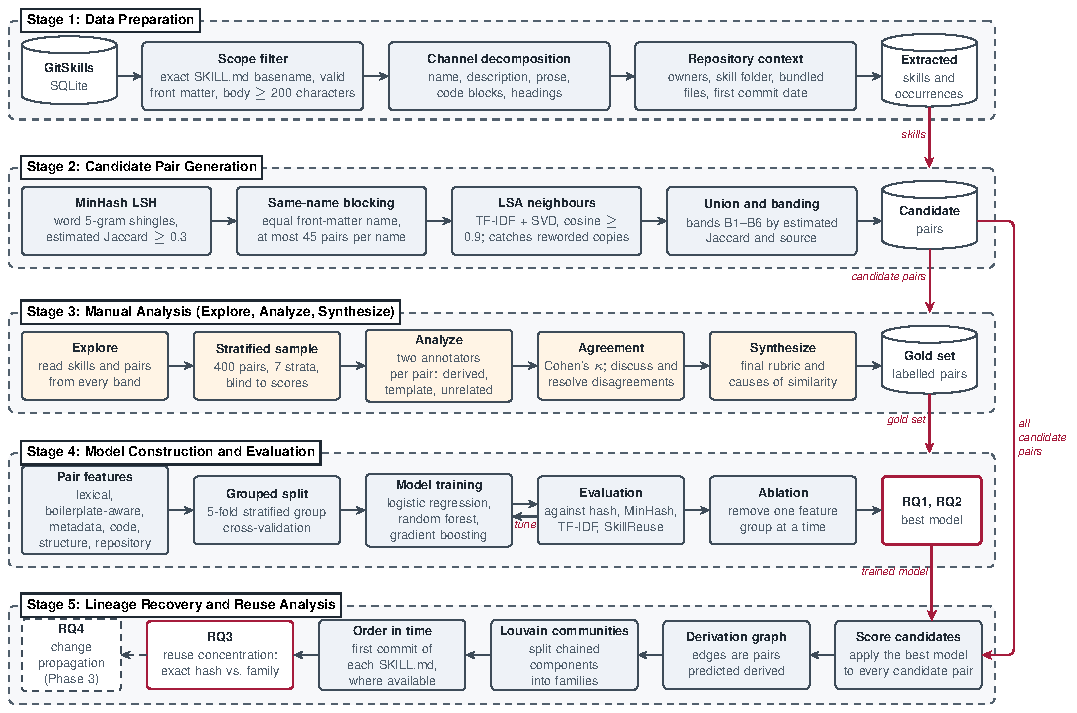
\includegraphics[width=\textwidth]{figures/approach_overview.pdf}
  \caption{Approach overview. Orange boxes are manual steps; boxes with a red outline answer
  our research questions. Stage~5 reads right to left, because it starts from the trained
  model and the full set of candidate pairs.}
  \label{fig:overview}
\end{figure*}

\paragraph{Stage 1: Data preparation.} We extract the working set described in
Section~\ref{sec:dataset} and split every skill into its name, description, prose, code
blocks, and headings, together with its repository context.

\paragraph{Stage 2: Candidate pair generation.} Comparing every pair of the
\ResWorkContents{} skills would take about 60 million comparisons, and more than a trillion
on the full dataset. We therefore score only pairs proposed by at least one of three
inexpensive blockers. First, MinHash locality-sensitive hashing~\cite{broder1997resemblance}
over word 5-gram shingles of the body (128 permutations) proposes pairs whose estimated
Jaccard similarity is at least 0.3. Second, same-name blocking proposes distinct contents
that carry the same normalised front-matter name, capped at 45 pairs per name so that
common names such as \texttt{code-review} do not dominate. Third, nearest neighbours in a
latent semantic analysis (LSA) space~\cite{deerwester1990lsa}, built from TF-IDF vectors of
the body reduced to 128 dimensions, propose each skill's three closest skills when their
cosine is at least 0.9; this catches reworded copies that share few exact shingles. Together
the blockers propose \ResCandTotal{} candidate pairs, which we assign to bands by estimated
Jaccard similarity $J$ or by the blocker that found them (Table~\ref{tab:bands}).

\begin{table}[t]
\caption{Similarity bands of candidate pairs and of the labelled sample.}
\label{tab:bands}
\small
\begin{tabular}{llrr}
\toprule
Band & Definition & Candidates & Labelled \\
\midrule
B1 & $J \geq 0.9$ & \ResBandOne & \ResSampleOne \\
B2 & $0.7 \leq J < 0.9$ & \ResBandTwo & \ResSampleTwo \\
B3 & $0.5 \leq J < 0.7$ & \ResBandThree & \ResSampleThree \\
B4 & $0.3 \leq J < 0.5$ & \ResBandFour & \ResSampleFour \\
B5 & same name, $J < 0.3$ & \ResBandFive & \ResSampleFive \\
B6 & LSA neighbour, $J < 0.3$ & \ResBandSix & \ResSampleSix \\
B7 & random pair (not a candidate) & -- & \ResSampleSeven \\
B0 & other LSH match, $J < 0.3$ & \ResBandZero & 0 \\
\midrule
 & Total & \ResCandTotal & \ResSampleTotal \\
\bottomrule
\end{tabular}
\end{table}

\paragraph{Stage 3: Manual analysis.} We followed the three steps of explore, analyse, and
synthesise.

\emph{Explore.} We first read a random set of skills, the most-copied contents, and candidate
pairs from every band to learn why skills resemble each other.
\tbd{State what you read, e.g., ``each of us read 25 skills and 20 pairs''.}
% VERIFY these examples during your own exploration; all of them occur in the official sample.
Much of the similarity in the middle bands turned out to come from shared scaffolding rather
than copying. Examples include a catalog of machine-generated skills whose names follow the
pattern \texttt{u02156-...} and whose texts differ in a few substituted words, integration
skills for many different applications that wrap the same Rube MCP (Composio) boilerplate, and
a series of German legal-practice skills that repeat the same checklist lines. Conversely,
many same-name pairs, such as two skills called \texttt{code-review}, were written
independently. These observations led to our three-class labelling scheme.

\emph{Analyse.} We drew a stratified sample of \ResSampleTotal{} pairs across the bands of
Table~\ref{tab:bands}, including \ResSampleSeven{} random pairs that no blocker proposed as
easy negatives. To keep the sample diverse, a skill appears in at most two pairs and a name
in at most four. The left--right order of each pair is randomised, and annotators never see
similarity scores or bands. Two team members labelled each pair independently in a
side-by-side diff viewer, following a written rubric that adapts the criterion Gao et al.\
used to validate their reuse links~\cite{gao2026registry}. A pair is \emph{derived} when the
skills share distinctive content that is unlikely to be written twice independently:
verbatim or lightly reworded passages, or the same task-specific steps, examples, commands,
paths, or configuration values; renamed and translated copies count as derived. A pair is a
\emph{template} pair when the overlap is limited to generic scaffolding while the
task-specific instructions differ. Otherwise it is \emph{unrelated}; sharing a topic alone is
not derivation. We measured agreement with Cohen's $\kappa$~\cite{cohen1960kappa} and resolved
disagreements in discussion.

\emph{Synthesise.} We revised the rubric with the cases that caused disagreement and grouped
the reasons pairs looked similar into a short list of causes
\tbd{list your categories, e.g., copy-and-edit, generator template, catalog house style,
one author's personal template, translation}. The resulting gold set contains
\ResGoldPairs{} pairs: \ResGoldDerived{} derived, \ResGoldTemplate{} template, and
\ResGoldUnrelated{} unrelated.

\paragraph{Stage 4: Model construction and evaluation.} For each pair we compute 19 features
in six groups (Table~\ref{tab:features}). The boilerplate-aware group is specific to our
problem. We normalise every line of a skill (lower case, list markers removed, whitespace
collapsed; at least 20 characters containing a letter) and call a line \emph{boilerplate} when
it appears in skills carrying at least \ResBoilerK{} different front-matter names; the working
set contains \ResBoilerLines{} such lines. A widely copied skill usually keeps its name, so
its lines stay distinctive, while scaffold lines recur under many unrelated names. Derived
variants should therefore share distinctive lines, and template siblings mostly boilerplate.
We train logistic regression, random forest, and gradient boosting classifiers with balanced
class weights and evaluate them with five-fold stratified group cross-validation, so that no
skill appears in both a training and a test fold (Section~\ref{sec:setup}).

\begin{table}[t]
\caption{Pair features used by our classifier.}
\label{tab:features}
\small
\begin{tabular}{>{\raggedright\arraybackslash}p{0.22\columnwidth}>{\raggedright\arraybackslash}p{0.70\columnwidth}}
\toprule
Group & Features \\
\midrule
Lexical & Jaccard and containment of word 5-gram shingles; TF-IDF cosine of the bodies;
normalised edit similarity of the first 5,000 characters \\
Boilerplate-aware & Jaccard and containment of distinctive lines; Jaccard of boilerplate
lines; share of shared lines that are boilerplate \\
Metadata & names equal; name similarity; TF-IDF cosine of the descriptions \\
Code & Jaccard of identifier tokens in code blocks; both skills contain code \\
Structure & similarity of heading sequences; length ratio; heading-count ratio \\
Repository & a shared owner; same skill-folder name; Jaccard of bundled file names \\
\bottomrule
\end{tabular}
\end{table}

\paragraph{Stage 5: Lineage recovery and reuse analysis.} We train the best model from
Stage~4 on all gold pairs and apply it to every candidate pair. Pairs predicted as derived
become edges of a derivation graph. Instead of taking connected components, which chain
unrelated skills together through a few bridging edges, we split the graph into families with
Louvain community detection~\cite{blondel2008louvain}. Where both skills of a derived pair have
commit history, the earlier first commit of \texttt{SKILL.md} gives the pair a direction.
Finally, we compare how concentrated reuse is when counted by exact hash and by family (RQ3).
Phase~3 will use the families to study change propagation (RQ4).
